\section{Introduction}
I have spent the majority of my time this week trying my Long - Short Term Memory network with features extracted from Places365's pre-trained ResNet18, learning how to implement LSTM in TensorFlow.

\section{Places365 Caption}
This week I also run Places365 on images to analyze scene categories and attributes. And I concatenated 10 most relevant attributes structuring caption for a concrete image. Finally we tried to used that caption as input of any Convolutional Neural Network to predict images' memorabilities. I rewrote the source code and it could be found \href{https://gitlab.com/tlvu2697/mit--csail--places365}{here on my GitLab.}

\section{TensorFlow LSTM Classification Network}
\subsection{Architecture}
\begin{figure}[!ht]
\centering
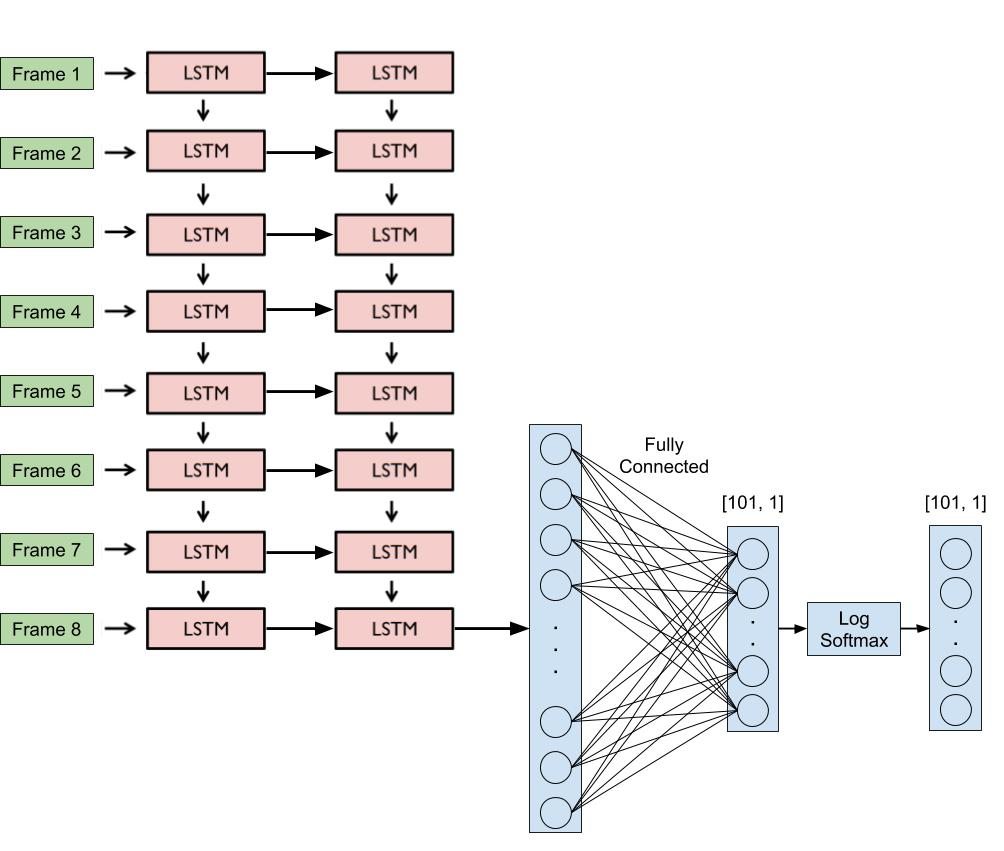
\includegraphics[width=\textwidth]{week11-lstmclassification-tf-v1.jpg}
\caption{Long - Short Term Memory Network Architecture.}
\end{figure}

This week I tried to implement Long - Short Term Memory network using TensorFlow library. I finally figured out what was the definition of graph and session term in TensorFlow. I also learnt some new TensorFlow functionalities for example Graph, Session, DropoutWrapper, BasicLSTMCell, MultiRNNCell, AdamOptimizer and argmax.

I re-designed my LSTM network using TensorFlow library and the figure below would demonstrate clearly how my network was. I used a stack of 2 LSTM cells sequences and only took the last LSTM cell's output for my Fully - connected layer. In each version I changed some hyper parameters to figure out whether I could increase the accuracy of not.

\subsection{Training on Dev-Set (extracted by ResNet50)}
\subsubsection{Strategy}
This times I broke the problem into the classification problem of 101 cate-gories. Because I thought this dataset was pretty small for deeplearning so I splitted the provided Dev-Set for this challenge into two parts, since the Dev-Set had 8000 videos, I picked \textbf{\emph{7000}} videos for training and \textbf{\emph{1000}} videos for testing.

\subsubsection{Version 1}
In this version, I trained a batch of size \textbf{\emph{128}} at once, with \textbf{\emph{512}} LSTM units for each LSTM cell and \textbf{\emph{7000}} iterations.

\begin{figure}[!ht]
\centering
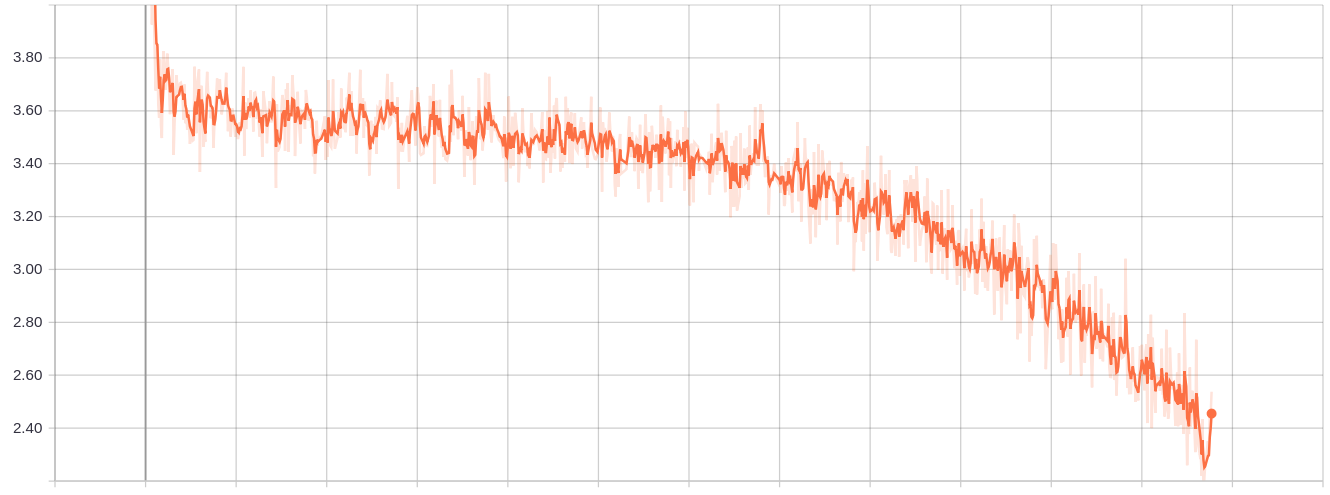
\includegraphics[width=\textwidth]{week11-resnet50-v1-loss.png}
\caption{Loss over Epoch.}
\end{figure}

\begin{figure}[!ht]
\centering
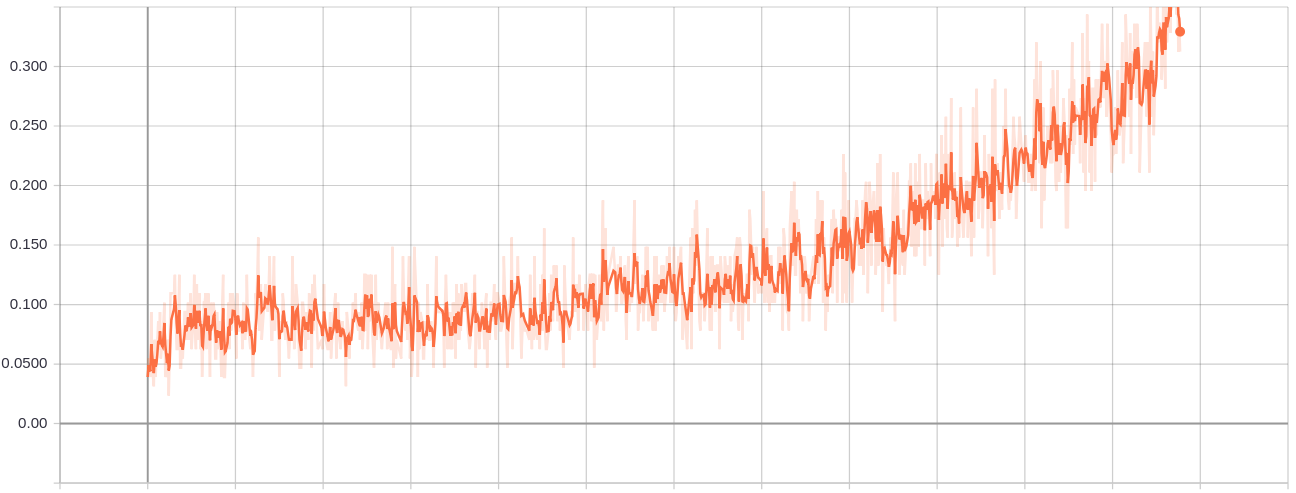
\includegraphics[width=\textwidth]{week11-resnet50-v1-accuracy.png}
\caption{Accuracy over Epoch.}
\end{figure}

After 7000 iterations, the loss value was \textbf{\emph{2.5}} and the accuracy value was \textbf{\emph{0.3}}. But from my perspective view, the loss and accuracy were both turbulent so lately I moved to another version with some hyper-parameter changed. After performing test on the \textbf{\emph{train set}}, I got the Spearman Rank Correlation of \textbf{\emph{0.37}}; on \textbf{\emph{test set}}, the Spearman Rank Correlation was just \textbf{\emph{0.05}}.

\subsubsection{Version 1.1}
In this revamp version, I trained a batch of size \textbf{\emph{512}} at once, with \textbf{\emph{1024}} LSTM units for each LSTM cell and \textbf{\emph{7000}} iterations.

\begin{figure}[!ht]
\centering
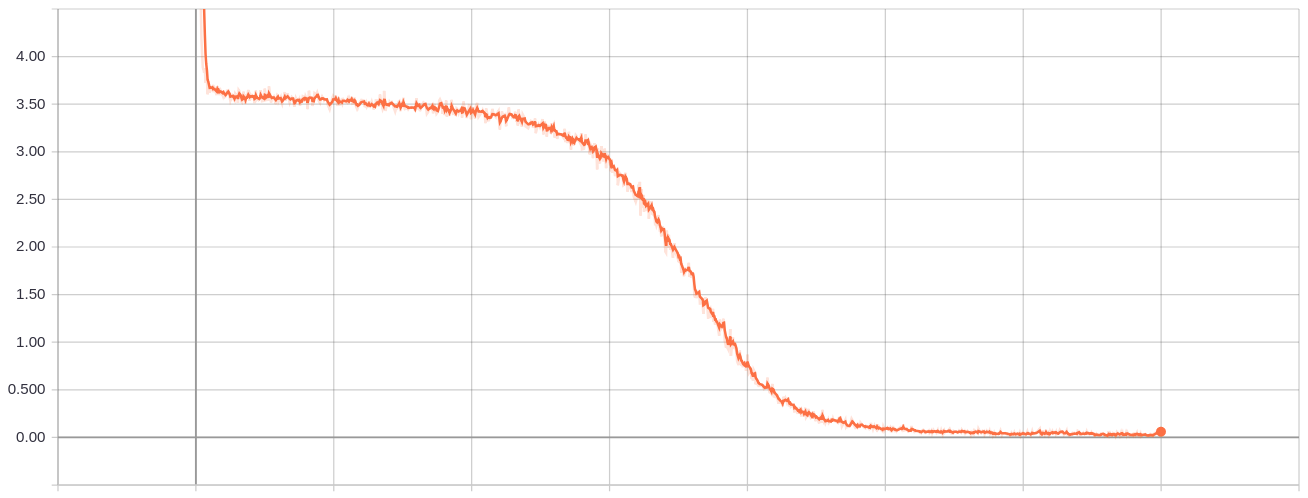
\includegraphics[width=\textwidth]{week11-resnet50-v2-loss.png}
\caption{Loss over Epoch.}
\end{figure}

\begin{figure}[!ht]
\centering
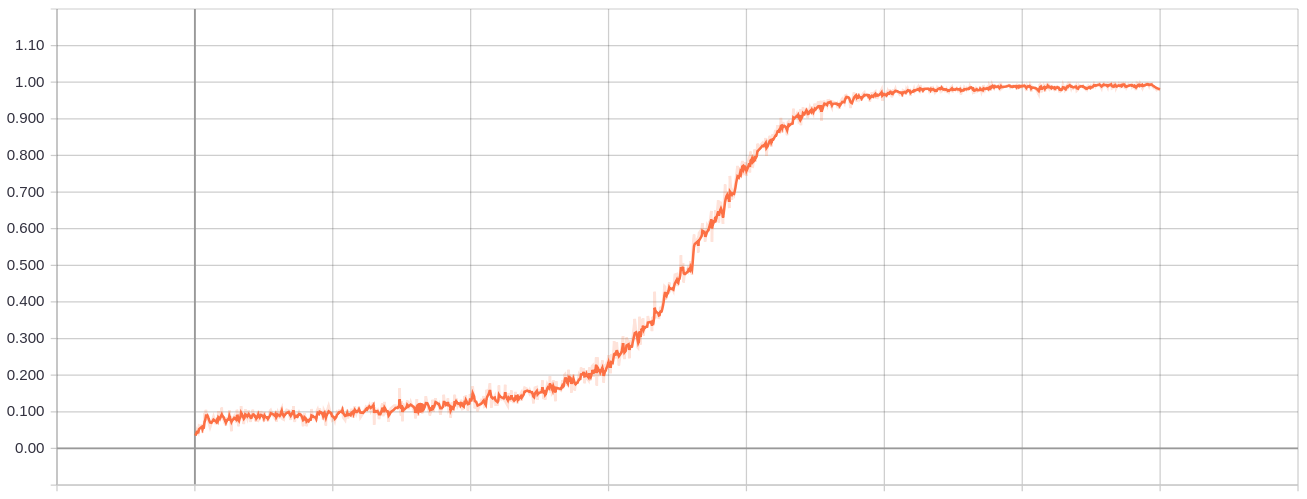
\includegraphics[width=\textwidth]{week11-resnet50-v2-accuracy.png}
\caption{Accuracy over Epoch.}
\end{figure}

After 7000 iterations, the loss value was \textbf{\emph{0.06}} and the accuracy value was \textbf{\emph{0.98}}. But from my perspective view, the loss and accuracy were both turbulent so lately I moved to another version with some hyper-parameter changed. After performing test on the \textbf{\emph{train set}}, I got the Spearman Rank Correlation of \textbf{\emph{0.98}}; on \textbf{\emph{test set}}, the Spearman Rank Correlation was just \textbf{\emph{0.03}}. This result seemed to be the consequence of overfitting. I thought 7000 iterations was not a good number.

\subsection{Training on Dev-Set (extracted by Places365)}
\subsubsection{Strategy}
I also broke the problem into the classification problem of 101 cate-gories. I first passed all of my input through Places365's pre-trained ResNet18 network and used those features as input of my LSTM network. The features extracted by ResNet18 had the dimension of \textbf{\emph{512}}. I aslo picked \textbf{\emph{7000}} videos for training and \textbf{\emph{1000}} videos for testing too.

\subsubsection{Version 1}
In this version, I trained a batch of size \textbf{\emph{128}} at once, with \textbf{\emph{256}} LSTM units for each LSTM cell and \textbf{\emph{7000}} iterations.

\begin{figure}[!ht]
\centering
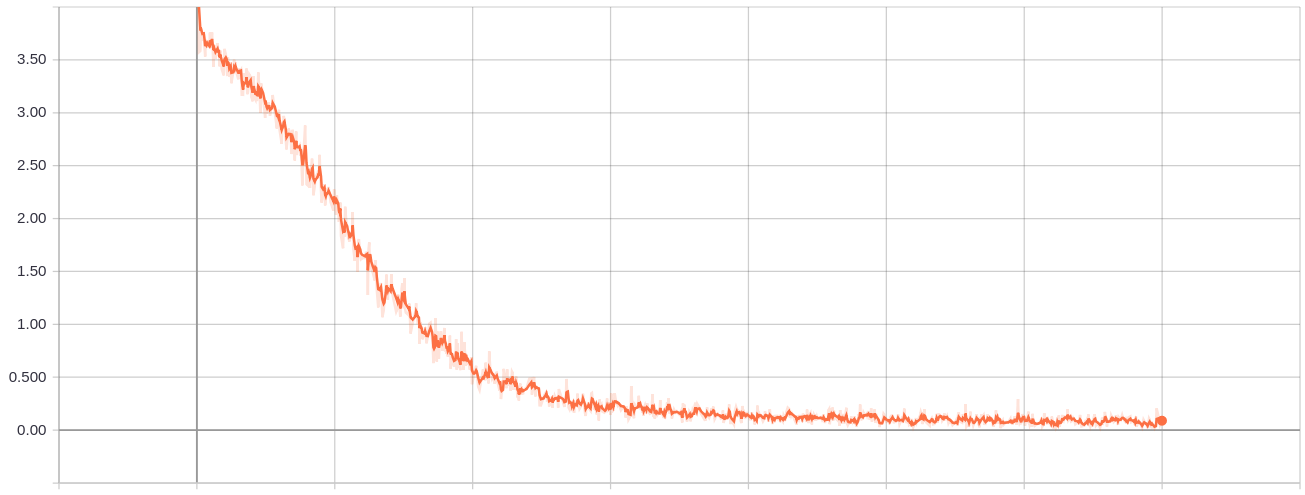
\includegraphics[width=\textwidth]{week11-places365-loss.png}
\caption{Loss over Epoch.}
\end{figure}

\begin{figure}[!ht]
\centering
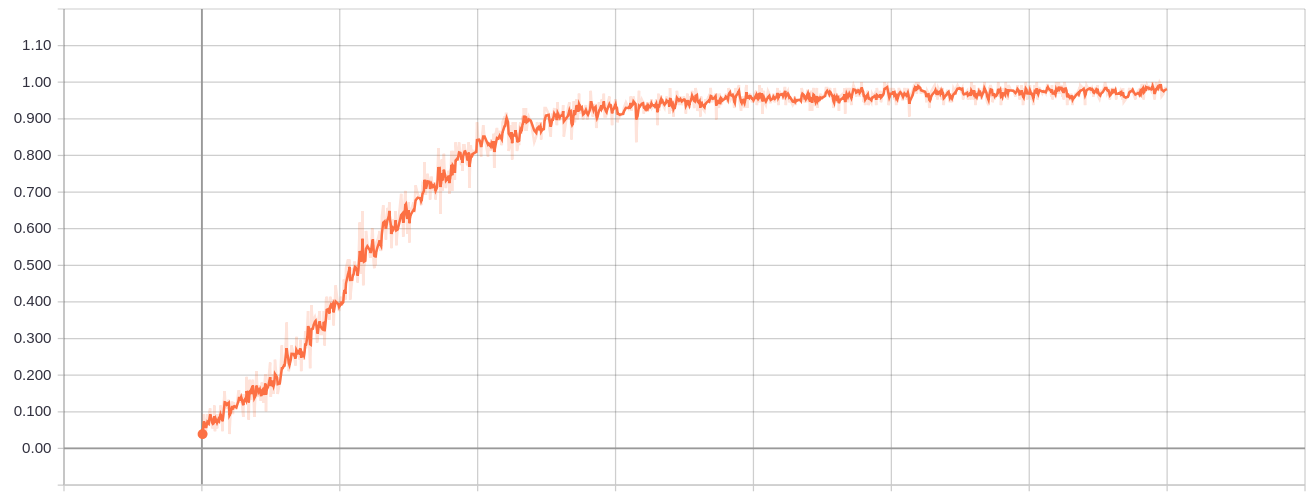
\includegraphics[width=\textwidth]{week11-places365-accuracy.png}
\caption{Accuracy over Epoch.}
\end{figure}

After 30000 iterations, the loss value was \textbf{\emph{0.09}} and the accuracy value was \textbf{\emph{0.98}}. But from my perspective view, the loss and accuracy were both turbulent so lately I moved to another version with some hyper-parameter changed. After performing test on the \textbf{\emph{train set}}, I got the Spearman Rank Correlation of \textbf{\emph{0.97}}; on \textbf{\emph{test set}}, the Spearman Rank Correlation was just \textbf{\emph{0.07}}. This result also seemed to be the consequence of overfitting. I should decrease the number of iterations in the next version.